% Provenance (never printed): see sources/outline_sources.md (Year 1: the carbonate factory;
% reefs and platforms; pelagic oozes and the carbonate compensation depth; siliceous oozes;
% evaporite sequences). Exercise and problem values in the Book 3 scratch calculator
% calc/ch22.py; figure data from figdata/bachelor-1/evaporation.py and ccd_flank.py.
% Calcite, aragonite and dolomite are ch. 7's; the depth--age law ch. 13's; salinity Book 1's
% (g8); limestone Book 1's (g6, prose); the carbonate system and alkalinity the chemistry and
% biology books' (recalled, never defined). The subsidence of volcanic islands under reefs is
% the Year 2 volume's (oceanic islands); diagenesis (dolomitisation, chert, gypsum to
% anhydrite) is ch. 23's; upwelling ch. 29's.
\chapter{Carbonaat-, kiezel- en verdampingssedimenten}\label{ch:b1:chemical-biogenic-sediments}

De witte kliffen van krijt die tegenover elkaar liggen over de smalle zee tussen Engeland en Frankrijk, lijken de gewoonste van alle gesteenten. Onder de elektronenmicroscoop blijken zij uit talloze kleine plaatjes calciet te bestaan, afgestoten door eencellige algen die in de zee dreven die de streek bedekte. Een \omterm{def:b1:chemical-biogenic-sediments:reef}{rif} dat vanuit een boot wordt gezien, is hetzelfde verhaal aan het andere eind van de schaal: een kalksteen in wording, gebouwd door koralen en algen die calcium en carbonaat uit het water halen en ze in steen omzetten. Niet alle sedimenten worden meegevoerd; veel ontstaan op de plaats waar zij liggen, door levende wezens of door het water zelf terwijl het verdampt. Dit hoofdstuk volgt de drie grote families van deze sedimenten, carbonaten, \omterm{def:b1:chemical-biogenic-sediments:ooze}{kiezelslijken} en \omterm{def:b1:chemical-biogenic-sediments:evaporite}{verdampingsgesteenten}, van de scheikunde van de zee die ze voedt tot de gesteenten die ze achterlaten.

\begin{recall}
Kalksteen is een sedimentair gesteente van calciet, vaak uit schelpen, en het bruist in verdund zuur (Boek~1, klas~6). Calciet en aragoniet zijn de twee \omterm{def:b1:rock-forming-minerals:polymorph}{polymorfen} van \ce{CaCO3}, met dichtheden van \qty{2.71}{g.cm^{-3}} en \qty{2.93}{g.cm^{-3}}, en dolomiet \ce{CaMg(CO3)2}, met dichtheid \qty{2.84}{g.cm^{-3}}, is het carbonaat van calcium en magnesium (\cref{ch:b1:rock-forming-minerals}). Het zoutgehalte van zeewater is de massa opgelost zout per kilogram ervan (Boek~1, klas~8). In water zijn koolstofdioxide, waterstofcarbonaat- en carbonaationen met zuur-base-evenwichten verbonden, en de alkaliniteit meet de basen die waterstofionen kunnen opnemen (de scheikundeboeken); het carbonaatsysteem van de oceaan neemt deel aan de koolstofkringloop (de biologieboeken). De zeebodem verdiept met de leeftijd als $d = d_r + C\sqrt t$ (\cref{thm:b1:rifts-ridges-margins:depth-age}).
\end{recall}
% ledger: webmineral:polymorphs, hom:calcite, webmineral:others

\section{De carbonaatfabriek}\label{sec:b1:chemical-biogenic-sediments:factory}

Zeewater bevat calcium en opgelost anorganisch koolstof, vooral als waterstofcarbonaat. Calciumcarbonaat vormt zich daaruit door de reacties
\[
\ce{Ca^2+ + 2 HCO3- -> CaCO3 + CO2 + H2O}, \qquad
\ce{Ca^2+ + CO3^2- -> CaCO3},
\]
de eerste, die voor elk afgezet carbonaatmolecuul een molecuul koolstofdioxide vrijmaakt. Warm oppervlaktewater van de tropen is oververzadigd in calciumcarbonaat, maar het slaat zelden vanzelf neer: vrijwel alles wordt door levende wezens gemaakt, die de energie betalen om hun schelpen en skeletten te bouwen en het \omterm{def:b1:rock-forming-minerals:mineral}{mineraal} dat zij gebruiken beheersen. Koralen en groene algen bouwen aragoniet; rode algen en veel foraminiferen bouwen calciet, een deel ervan rijk aan magnesium; weekdieren gebruiken een of beide.

\begin{definition}[Carbonaatfabriek]\label{def:b1:chemical-biogenic-sediments:factory}
De \emph{carbonaatfabriek}\index{carbonaatfabriek} van een zee is de verzameling van organismen en processen die calciumcarbonaatsediment produceren op de plaats waar het wordt gevonden, in plaats van het elders vandaan te halen. Haar producten zijn skeletkorrels (hele of gebroken schelpen en skeletten), carbonaatmodder, bedekte korrels en de stijve raamwerken van riffen.
\end{definition}

De rijkste fabriek werkt in warm, helder, ondiep en zonnig water, ver van de modder van rivieren, die de producenten zou begraven en het licht zou verduisteren dat de algen nodig hebben. Haar sediment wordt door de zeebodem zelf gemaakt: koraal- en algenpuin, de schelpen van weekdieren en van de eencellige foraminiferen die op de bodem leven, en naalden van aragoniet die door groene algen worden afgestoten en die als kalkmodder bezinken. Waar het water wordt geroerd en oververzadigd is, krijgen korrels die door golven en getijden worden rondgerold, lagen carbonaat aangroeien, laag na laag, rond een kern, een zandkorrel of een schelfragment, tot ronde oolieten (\cref{def:b1:chemical-biogenic-sediments:reef}). Een tweede fabriek werkt in de open oceaan, ver van elke kust: het plankton dat in de zonverlichte oppervlaktelaag leeft, bouwt kleine calcietschelpjes en -plaatjes die naar de diepzeebodem regenen (\cref{sec:b1:chemical-biogenic-sediments:oozes}).
% ledger: og:carbonates

Hoe snel een fabriek bouwt, wordt gemeten door haar carbonaatbudget: de massa carbonaat die per vierkante meter per jaar wordt geproduceerd en op zijn plaats gehouden, na de verliezen door boorende organismen, grazers en de golven. Met een massabalans wordt het een verticale groeisnelheid.

\begin{proposition}[Aanwas uit een carbonaatbudget]\label{prop:b1:chemical-biogenic-sediments:accretion}
Laat een zeebodem per oppervlakte-eenheid en per tijdseenheid de netto massa $G$ calciumcarbonaat op zijn plaats houden, als een afzetting waarvan de vaste korrels de dichtheid $\rho_s$ hebben en waarvan de porositeit, het deel van het volume dat door poriën wordt ingenomen, $\phi$ is. Dan stijgt de bodem met de snelheid
\[
a = \frac{G}{\rho_s\,(1-\phi)}.
\]
\end{proposition}

\begin{proof}
In de tijd $\mathrm dt$ ontvangt een oppervlakte-eenheid de massa $G\,\mathrm dt$ van vast carbonaat, dat het volume $G\,\mathrm dt/\rho_s$ van korrels vult. Deze korrels maken het deel $1-\phi$ van de nieuwe laag uit, waarvan de dikte dus $G\,\mathrm dt/(\rho_s(1-\phi))$ is. Het delen door $\mathrm dt$ geeft $a$.
\end{proof}

Het product $\rho_s(1-\phi)$ is de droge volumieke dichtheid van de afzetting. Op de riffen van de Chagos-archipel in de Indische Oceaan hadden 28 riffen die in 2015 zijn gemeten een gemiddeld budget van \qty{3.7}{kg} \ce{CaCO3} per vierkante meter per jaar; de riffen die door vertakte \emph{Acropora}-koralen werden beheerst, hadden \qty{8.4}{kg}, en groeiden met ongeveer \qty{4.2}{mm} per jaar. Met de propositie betekenen deze twee getallen samen een droge volumieke dichtheid van \qty{2000}{kg.m^{-3}}, dat is een rifraamwerk met ongeveer een derde poriënruimte (\cref{exo:b1:chemical-biogenic-sediments:3}). Dezelfde riffen hadden bij de opwarmingsgebeurtenis van 1998 meer dan negen tiende van hun koralen verloren, en hun budgetten laten zien hoe snel een \omterm{def:b1:chemical-biogenic-sediments:reef}{rif} zich kan herstellen.
% ledger: perry:chagos

\section{Riffen en platforms}\label{sec:b1:chemical-biogenic-sediments:reefs}

Waar de fabriek een stijf raamwerk bouwt, kan het uit de zeebodem tegen de golven oprijzen.

\begin{definition}[Rif, carbonaatplatform, oöide]\label{def:b1:chemical-biogenic-sediments:reef}
Een \emph{rif}\index{rif} is een carbonaatopbouw waarvan het raamwerk van organismen, koralen, algen of andere, ter plaatse gegroeid en met elkaar verbonden en verkit, boven de omringende zeebodem uitsteekt en de golven weerstaat. Een \emph{carbonaatplatform}\index{carbonaatplatform} is een dik lichaam van ondiep carbonaat waarvan de vlakke top dicht bij het zeeniveau ligt en dat wordt begrensd door een helling naar dieper water. Een \emph{oöide}\index{oöide} is een ronde korrel van zandgrootte die uit concentrische lagen calciumcarbonaat bestaat, gegroeid rond een kern terwijl zij in bewogen water rolde; een gesteente dat uit oöïden bestaat, is een oöliet.
\end{definition}
% ledger: og:carbonates

Moderne koraalriffen komen in drie soorten voor, genoemd door de zeevaarders die ze in kaart brachten lang voordat iemand er doorheen boorde. Een \emph{kustrif} hangt aan de kust van een eiland of een continent. Een \emph{barrièrerif} is van het land gescheiden door een lagune, die breed kan zijn en tientallen meters diep: de barrière voor het noordoosten van Australië loopt, met onderbrekingen, bijna \qty{1600}{km} ver en omsluit een zee van 10 tot 25 vadem diep, ongeveer 18 tot \qty{46}{m}. Een \emph{atol} is een ring van \omterm{def:b1:chemical-biogenic-sediments:reef}{rif}, met lage eilanden van koraalzand, rond een lagune zonder enig land erin.

\begin{omfigure}
\begin{tikzpicture}[font=\footnotesize, scale=0.72]
% three reef types in cross-section (schematic): a volcanic cone y = 2 - s - 0.75|x - 4|
% subsided by s (0, 0.8, 1.6), sea level at y = 1; the reef grows up from its first
% position, the foot of the fringing reef at (2, 0.5) moving down with the cone
\foreach \s/\yo/\lab/\name in {0/0/a/kustrif, 0.8/-3.8/b/barrièrerif, 1.6/-7.6/c/atol} {
  \begin{scope}[yshift=\yo cm]
    \begin{scope}
      \clip (0,-1.3) rectangle (8,2.3);
      \fill[omSea] (0,-1.3) rectangle (8,1.0);
      \draw[lith basalt] (-1,2-\s-3.75) -- (4,2-\s) -- (9,2-\s-3.75) -- cycle;
    \end{scope}
    \draw[omSea!60!black] (0,1.0) -- (8,1.0);
    \node[anchor=west, font=\scriptsize] at (8.05,1.0) {zeeniveau};
    \node[anchor=west] at (0,2.05) {(\lab) \name};
    \draw[black!70] (1.05,1.55) node[anchor=east, font=\scriptsize] {rif} -- (2.2,1.02);
  \end{scope}
}
% (a) fringing reef: wedges against the shore
\fill[lith reef limestone, draw=black!70] (2.0,0.5) -- (2.15,1.0) -- (2.667,1.0) -- cycle;
\fill[lith reef limestone, draw=black!70] (6.0,0.5) -- (5.85,1.0) -- (5.333,1.0) -- cycle;
\node[anchor=west, font=\scriptsize] at (4.9,1.75) {vulkanisch eiland};
% (b) barrier reef: the cone has sunk by 0.8, the reef has grown up, a lagoon opens
\begin{scope}[yshift=-3.8cm]
  \fill[lith reef limestone, draw=black!70] (2.0,-0.3) -- (2.15,1.0) -- (2.6,1.0) -- (2.55,0.1125) -- cycle;
  \fill[lith reef limestone, draw=black!70] (6.0,-0.3) -- (5.85,1.0) -- (5.4,1.0) -- (5.45,0.1125) -- cycle;
  \draw[black!70] (3.2,0.85) -- (3.45,1.55) node[anchor=south west, font=\scriptsize, inner sep=1pt] {lagune};
\end{scope}
% (c) atoll: the cone has sunk by 1.6 and is drowned; the reef ring encloses a lagoon
\begin{scope}[yshift=-7.6cm]
  \fill[lith limestone, draw=black!50] (2.55,-0.6875) -- (2.55,0.55) -- (5.45,0.55) -- (5.45,-0.6875) -- (4,0.4) -- cycle;
  \fill[lith reef limestone, draw=black!70] (2.0,-1.1) -- (2.15,1.0) -- (2.6,1.0) -- (2.55,-0.6875) -- cycle;
  \fill[lith reef limestone, draw=black!70] (6.0,-1.1) -- (5.85,1.0) -- (5.4,1.0) -- (5.45,-0.6875) -- cycle;
  \node[font=\scriptsize] at (4,0.78) {lagune};
  \node[font=\scriptsize, fill=omLithLime, inner sep=1pt] at (4,0.05) {lagunesediment};
\end{scope}
% photograph
\node[anchor=north west, inner sep=0] at (10.75,2.3) {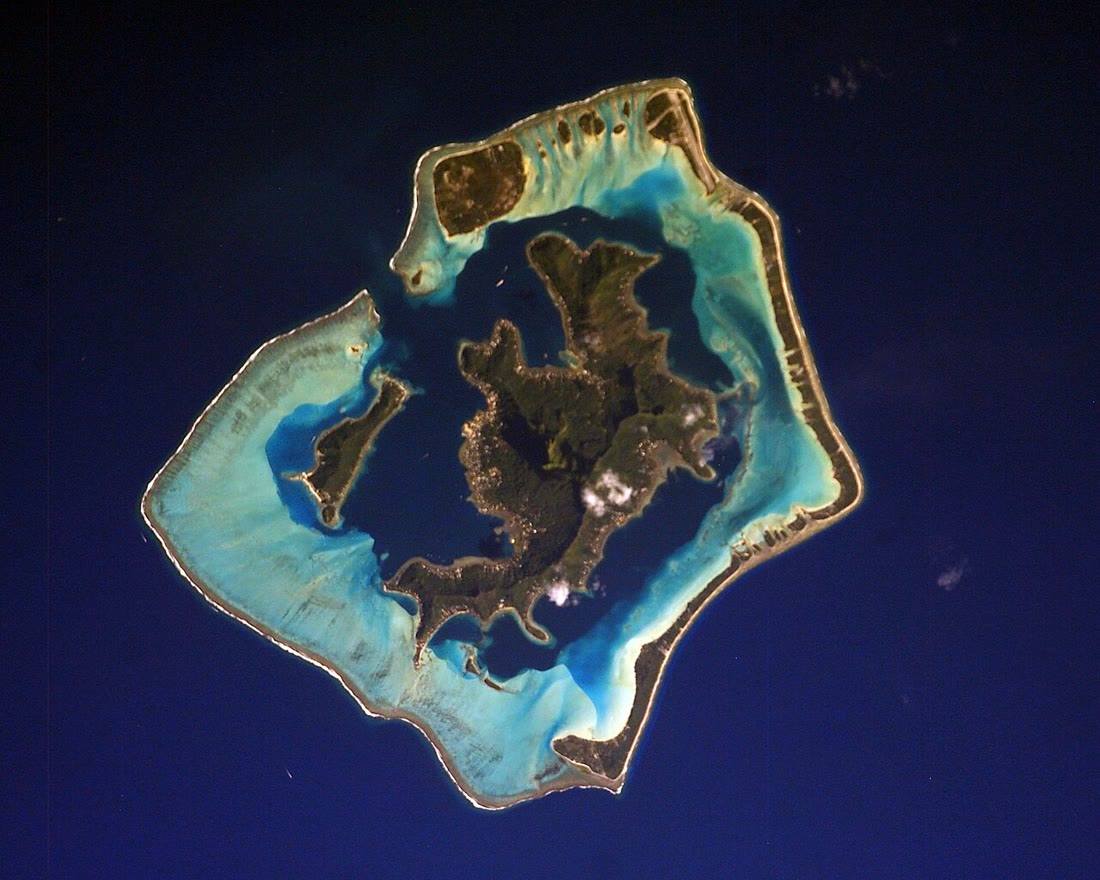
\includegraphics[height=6.9cm]{images/book3/b1-bora-bora.jpg}};
\end{tikzpicture}

{\small Links: de drie soorten koraalrif in doorsnede (schematisch, verticale schaal sterk overdreven), getekend zoals Darwin ze verklaarde: (a)~een \omterm{def:b1:chemical-biogenic-sediments:reef}{rif} dat een vulkanisch eiland omzoomt; (b)~het eiland is gezonken en het \omterm{def:b1:chemical-biogenic-sediments:reef}{rif}, dat omhoog groeit, is een barrière geworden die van de kust is gescheiden door een lagune; (c)~het eiland is uit het zicht gezonken en het \omterm{def:b1:chemical-biogenic-sediments:reef}{rif} is een atol rond een lagune met carbonaatsediment als bodem. Rechts: Bora Bora, een vulkanisch eiland in een lagune die door een barrièrerif is omsloten met lage eilanden erop, door een astronaut van het Internationaal Ruimtestation gefotografeerd op 19 maart 2003 (NASA, publiek domein, via Wikimedia Commons).}
\label{fig:b1:chemical-biogenic-sediments:reefs}
\end{omfigure}
% ledger: darwin:reefs, commons:bora-bora

\begin{history}[Riffen op zinkende fundamenten, 1837--1842]
Tijdens de reis van de \emph{Beagle} voer Charles Darwin tussen de riffen van de Stille en Indische Oceaan. Hij redeneerde vanuit één feit: riffbouwende koralen, concludeerde hij, gedijen in de gewone gevallen niet dieper dan tussen 20 en 30 vadem, ongeveer 37 tot \qty{55}{m}. Toch rijzen barrièrerifs en atollen uit diep water op, ver onder die grens. Hun fundamenten, betoogde hij, moeten gezonken zijn, traag genoeg om de koralen hun top aan het oppervlak te laten houden door omhoog te groeien: een \omterm{def:b1:chemical-biogenic-sediments:reef}{rif} dat een vulkanisch eiland omzoomt wordt een barrière wanneer het eiland erbinnen zinkt, en een atol wanneer het eiland is verdwenen. Hij las zijn theorie voor aan de Geological Society van Londen op 31 mei 1837 en publiceerde haar in 1842 in \emph{The Structure and Distribution of Coral Reefs}, met een kaart van alle riffen van de wereld gesorteerd naar de drie soorten. Waarom oceaaneilanden zinken, en hoe ver, is een kwestie van de afkoeling van de plaat eronder, die in Boek~4 wordt behandeld.
\end{history}
% ledger: darwin:reefs

Een \omterm{def:b1:chemical-biogenic-sediments:reef}{rif} overleeft alleen als zijn top in het ondiepe water blijft waar zijn bouwers leven. Het zeeniveau verandert, en het fundament kan zakken; wat telt is de som van de twee, de relatieve stijging van het zeeniveau.

\begin{proposition}[Bijhouden of verdrinken]\label{prop:b1:chemical-biogenic-sediments:keep-up}
Laat de top van een \omterm{def:b1:chemical-biogenic-sediments:reef}{rif} op de diepte $D_0$ onder het zeeniveau liggen en omhoog groeien met de snelheid $a$, terwijl het relatieve zeeniveau stijgt met de snelheid $r$, beide constant. Dan is de diepte van het water boven het \omterm{def:b1:chemical-biogenic-sediments:reef}{rif} na de tijd $t$
\[
D(t) = D_0 + (r - a)\,t .
\]
Als $a \ge r$ houdt het \omterm{def:b1:chemical-biogenic-sediments:reef}{rif} gelijke tred met de zee (wanneer $a > r$ bereikt zijn top het oppervlak, en kan hij van dan af alleen zijwaarts groeien); als $a < r$ raakt het achter, en als zijn bouwers niet dieper dan $D_{\max}$ kunnen leven, verdrinkt het na de tijd $(D_{\max} - D_0)/(r - a)$.
\end{proposition}

\begin{proof}
Meet de hoogten omhoog vanaf een vast merkteken op het fundament. De top van het \omterm{def:b1:chemical-biogenic-sediments:reef}{rif}
ligt op $h_0 + a t$ en het zeeoppervlak op $s_0 + r t$, dus is de diepte van het water boven
de top gelijk aan $D = (s_0 - h_0) + (r - a)t = D_0 + (r-a)t$. Wanneer $a > r$, bereikt $D$
nul op $t = D_0/(a-r)$ en kan het \omterm{def:b1:chemical-biogenic-sediments:reef}{rif} niet boven de zee groeien. Wanneer
$a < r$ groeit $D$ lineair en bereikt $D_{\max}$ wanneer $(r-a)t = D_{\max} -
D_0$.
\end{proof}

Een \omterm{def:b1:chemical-biogenic-sediments:reef}{rif} waarvan de top is verdronken, is niet meteen dood, maar het licht verzwakt, de bouwers veranderen en de fabriek vertraagt, zodat een \omterm{def:b1:chemical-biogenic-sediments:reef}{rif} dat achterraakt verder achterraakt: verdronken riffen en platforms, afgedekt met diepwatersediment, worden gevonden op de hellingen van veel oceaaneilanden en in de gesteentelaag.

Over miljoenen jaren bouwen de fabrieken \omterm{def:b1:chemical-biogenic-sediments:reef}{carbonaatplatforms}, dikke lichamen van ondiep carbonaat die groeien terwijl hun fundamenten zakken. Twee vormen komen steeds terug (zie de figuur hieronder). Een \emph{omrand plat} heeft een vlakke top, beschermd achter een rand van riffen en banken van oöïden aan zijn rand, die de golven breekt; erachter ligt een rustige lagune van kalkmodder, en ervoor een steile helling waar blokken en puin die van de rand zijn afgeslagen naar het bekken vallen. Een \emph{rampe} helt zeer zacht van de kust naar het bekken zonder knik: oöïdebanken en schelpbanken waar de golven de bodem roeren, dan lagen schelppuin die door stormen wordt weggespoeld, dan kalkmodder onder het bereik van de golven. Een omrand plat groeit vooral omhoog en naar buiten vanaf zijn rand, een rampe door zijn sedimentgordels landwaarts of zeewaarts te verplaatsen naarmate de zee stijgt of daalt.

\begin{omfigure}
\begin{tikzpicture}[font=\footnotesize, >={Stealth[length=4pt]}]
% (a) rimmed shelf and (b) ramp, schematic cross-sections
\begin{scope}
  \fill[omSea] (0,0.2) rectangle (7.2,2.0);
  \fill[lith limestone, draw=black!60] (0,0) -- (0,1.55) -- (4.3,1.55) -- (4.5,1.75) -- (4.9,1.75) -- (5.1,1.5) -- (6.4,0.35) -- (7.2,0.3) -- (7.2,0) -- cycle;
  \fill[lith reef limestone, draw=black!70] (4.3,1.55) -- (4.5,1.75) -- (4.9,1.75) -- (5.1,1.5) -- (4.8,1.05) -- (4.3,1.05) -- cycle;
  \draw[omSea!60!black] (0,2.0) -- (7.2,2.0);
  \node at (2.1,1.78) {lagune: kalkmodder};
  \node[anchor=south, align=center, font=\scriptsize] at (4.7,2.05) {rif-rand en\\ oöïdbanken};
  \node[anchor=west, font=\scriptsize] at (5.6,1.2) {helling: puin};
  \node[font=\scriptsize] at (6.75,0.75) {bekken};
  \node at (3.6,-0.35) {(a) omrand plat};
\end{scope}
\begin{scope}[xshift=8.0cm]
  \fill[omSea] (0,0.2) rectangle (7.2,2.0);
  \fill[lith limestone, draw=black!60] (0,0) -- (0,1.85) -- (7.2,0.55) -- (7.2,0) -- cycle;
  \draw[omSea!60!black] (0,2.0) -- (7.2,2.0);
  \draw[densely dashed, black!50] (0,1.6) -- (7.2,1.6) node[pos=1, anchor=south east, font=\scriptsize, inner sep=1pt] {golven bij mooi weer bereiken};
  \draw[densely dashed, black!50] (0,1.0) -- (7.2,1.0) node[pos=1, anchor=south east, font=\scriptsize, inner sep=1pt] {stormgolven bereiken};
  \node[anchor=south, font=\scriptsize] at (0.9,2.05) {oöïdbanken};
  \node[anchor=south, font=\scriptsize] at (3.4,2.05) {stormschelpbanken};
  \node[anchor=south, font=\scriptsize] at (6.1,2.05) {kalkmodder};
  \node at (3.6,-0.35) {(b) rampe};
\end{scope}
\end{tikzpicture}

{\small De twee vormen van \omterm{def:b1:chemical-biogenic-sediments:reef}{carbonaatplatform} (schematisch, hellingen sterk overdreven). (a)~Een omrand plat: een rand van riffen en oöïdebanken breekt de golven, achter ligt een rustige lagune van kalkmodder, en puin dat van de rand afvalt glijdt de helling af naar het bekken. (b)~Een rampe helt zacht van de kust naar het bekken, haar sedimenten gesorteerd naar de diepte die de golven bereiken.}
\label{fig:b1:chemical-biogenic-sediments:platforms}
\end{omfigure}

\section{Pelagische slijken en de carbonaatcompensatiediepte}\label{sec:b1:chemical-biogenic-sediments:oozes}

Ver van het land ontvangt de zeebodem bijna niets van de continenten behalve het fijnste door de wind aangevoerde stof. Wat er wel op valt, zijn de skeletten van het plankton dat in het zonverlichte water kilometers erboven leefde: de calcietplaatjes van coccolithoforen en de schelpen van foraminiferen, de opalen frustules van diatomeeën en de skeletten van radiolariën (verderop afgebeeld). De lange regen van coccolithen naar de zeebodem is het belangrijkste proces dat krijt en een groot deel van de kalksteen van de wereld maakt.
% ledger: nasa:coccoliths-b3, og:carbonates

\begin{definition}[Kalkslijk, kiezelslijk]\label{def:b1:chemical-biogenic-sediments:ooze}
Een slijk is een fijnkorrelig pelagisch sediment, in de open oceaan afgezet, meestal uit
skeletten van plankton. Het is een \emph{kalkslijk}\index{kalkslijk} wanneer die van calciumcarbonaat zijn, vooral coccolithen en foraminiferen, en een \emph{kiezelslijk}\index{kiezelslijk}
wanneer zij van opaal zijn, amorf gehydrateerd silica, vooral diatomeeën en radiolariën.
\end{definition}
% ledger: og:carbonates

\omterm{def:b1:chemical-biogenic-sediments:ooze}{Kalkslijken} bedekken ongeveer de helft van de zeebodem van de wereld, maar alleen boven een zekere diepte: beneden ongeveer \qty{4500}{m} verdwijnen zij. De schelpen houden daar niet op met vallen; zij lossen op. De diepe oceaan is koud en de druk is hoog, en de oplosbaarheid van calciet neemt met de diepte toe, vooral door de druk, terwijl de concentratie van carbonaationen in het water over het algemeen met de diepte afneemt (de scheikunde van deze evenwichten wordt uit de scheikundeboeken herinnerd). Beneden een zekere diepte is diep water onderverzadigd in calciet, en lossen de schelpen die de bodem bereiken sneller op naarmate zij dieper liggen.
% ledger: britannica:ccd, slotnick:ccd-definitions

\begin{omfigure}
\begin{tikzpicture}
\node[inner sep=0] (a) at (0,0) {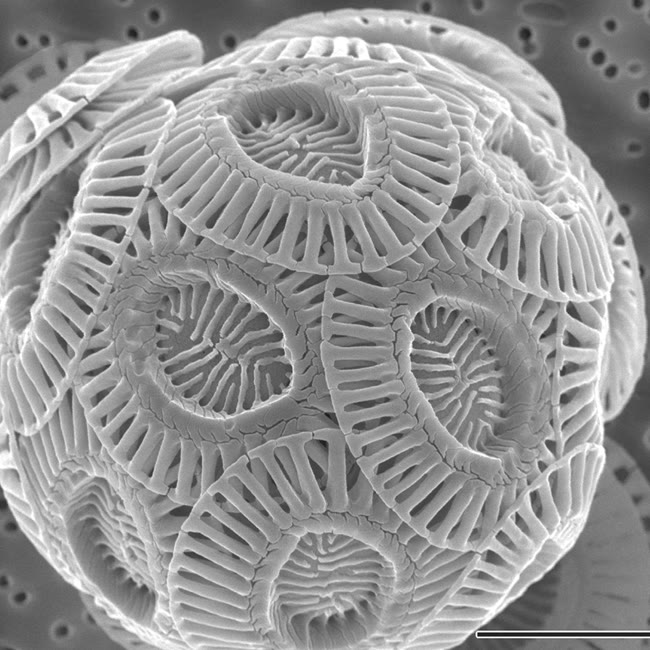
\includegraphics[height=4.3cm]{images/book3/b1-coccolithophore.jpg}};
\node[inner sep=0, anchor=west] (b) at ([xshift=0.25cm]a.east) {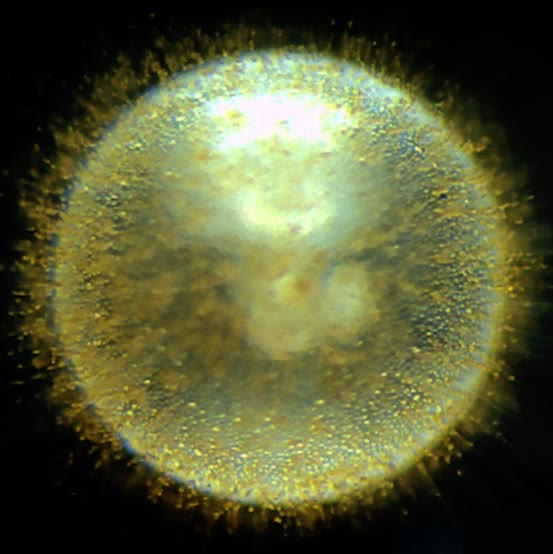
\includegraphics[height=4.3cm]{images/book3/b1-orbulina.jpg}};
\node[inner sep=0, anchor=west] (c) at ([xshift=0.25cm]b.east) {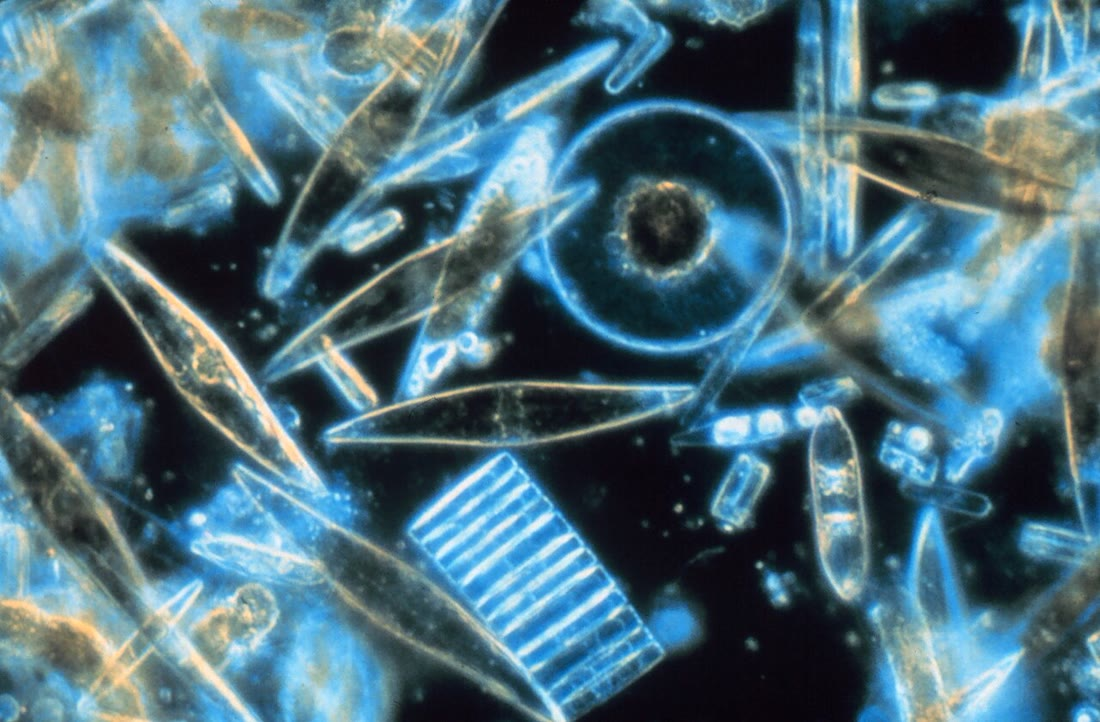
\includegraphics[height=4.3cm]{images/book3/b1-diatoms.jpg}};
\node[font=\footnotesize, anchor=north] at (a.south) {(a) een coccolithofoor};
\node[font=\footnotesize, anchor=north] at (b.south) {(b) een foraminifeer};
\node[font=\footnotesize, anchor=north] at (c.south) {(c) diatomeeën};
\end{tikzpicture}

{\small De makers van slijken. (a)~Een enkele cel van \emph{Emiliania huxleyi}, gepantserd met coccolithen, haar plaatjes van calciet (elektronenmicroscoop; Alison R.~Taylor, University of North Carolina Wilmington, CC~BY~2.5, via Wikimedia Commons). (b)~Een levende planktonische foraminifeer, \emph{Orbulina universa}, met haar calcietschaal omgeven door stekels (lichtmicroscoop; H.~Takagi en co-auteurs, 2019, CC~BY~4.0, via Wikimedia Commons). (c)~Levende diatomeeën uit het zee-ijs van McMurdo Sound, Antarctica, elk in haar frustule van opaal (lichtmicroscoop; Gordon T.~Taylor, Stony Brook University, NOAA, publiek domein, via Wikimedia Commons).}
\label{fig:b1:chemical-biogenic-sediments:plankton}
\end{omfigure}
% ledger: commons:ehux, commons:orbulina, commons:diatoms-noaa

\begin{definition}[Lysoklien, carbonaatcompensatiediepte]\label{def:b1:chemical-biogenic-sediments:ccd}
Het \emph{lysoklien}\index{lysoklien} is de diepte in de oceaan waaronder de oplossing van calciet op de zeebodem voor het eerst zichtbaar wordt in het sediment en haar snelheid scherp toeneemt. De \emph{carbonaatcompensatiediepte}\index{carbonaatcompensatiediepte} (CCD) is de diepte waarop de snelheid van oplossing van calciet gelijk is aan de snelheid waarmee calciet op de zeebodem neerregent; daaronder hoopt zich geen calciumcarbonaat op. In de praktijk wordt zij gelegd waar het calciumcarbonaatgehalte van het oppervlaktesediment onder \qty{10}{\%} op gewichtsbasis zakt.
\end{definition}
% ledger: slotnick:ccd-definitions

De CCD ligt gewoonlijk honderden meters onder de \omterm{def:b1:chemical-biogenic-sediments:ccd}{lysoklien}. Zij is geen vast niveau: zij wordt bepaald door een evenwicht tussen aanvoer en oplossing, dus ligt zij dieper waar het plankton meer carbonaat produceert en waar het diepe water minder corrosief is. In de Atlantische Oceaan ligt zij ongeveer \qty{500}{m} dieper dan in de Stille Oceaan, het gevolg van zowel een grotere aanvoer van carbonaat als een tragere oplossing; binnen de westelijke Stille Oceaan alleen al ligt zij op ongeveer \qty{4000}{m} in het noordwesten en op ongeveer \qty{5100}{m} in het centrale deel. Aragoniet, oplosbaarder dan calciet, lost op nog ondiepere dieptes op. In de geologische tijd hebben veranderingen in de aanvoer, in de productiviteit en in de oplossing de CCD meer dan \qty{2000}{m} verplaatst.
% ledger: slotnick:ccd-definitions, britannica:ccd, zhang:ccd-west-pacific

\begin{method}[Het lysoklien en de CCD vinden]\label{met:b1:chemical-biogenic-sediments:ccd}
\begin{enumerate}
  \item Verzamel de bovenste paar centimeter sediment op plaatsen op verschillende diepte
        in één gebied, ver genoeg van land en van opwelling om verdunning door
        klei of door opaal klein te laten zijn.
  \item Meet het gewichtspercentage \ce{CaCO3} van elk monster en zet het uit
        tegen de waterdiepte.
  \item Het \omterm{def:b1:chemical-biogenic-sediments:ccd}{lysoklien} is de diepte waar het gehalte steil begint te dalen,
        en waar de schelpen de eerste tekenen van oplossing tonen (gebroken,
        geëtste foraminiferen).
  \item De CCD is de diepte waar het gehalte daalt tot \qty{10}{\%}: lees haar af
        door lineaire interpolatie tussen de twee monsters aan weerszijden.
\end{enumerate}
\end{method}

Op de flank van een middenoceanische rug is de zeebodem jong en ondiep nabij de as en zakt hij naarmate hij ouder wordt en zich verder verwijdert. Een stuk vloer dat boven de CCD is gevormd, verzamelt \omterm{def:b1:chemical-biogenic-sediments:ooze}{kalkslijk} tot het onder de CCD zakt; vanaf dan ontvangt het alleen wat niet oplost: het stof dat uit de lucht neerdaalt, ijzer- en mangaanoxiden, de tanden van vissen. Deze langzame, bruine afzetting is de rode klei van de diepe bekkens.

\begin{proposition}[De CCD oversteken]\label{prop:b1:chemical-biogenic-sediments:flank}
Laat de zeebodem van leeftijd $t$ liggen op de diepte $d(t) = d_r + C\sqrt t$
(\cref{thm:b1:rifts-ridges-margins:depth-age}), met een as van de rug op de diepte $d_r$
ondieper dan een \omterm{def:b1:chemical-biogenic-sediments:ccd}{carbonaatcompensatiediepte} $z_c$ die constant blijft. Dan passeert de vloer de CCD op de leeftijd
\[
t_c = \left(\frac{z_c - d_r}{C}\right)^2 ,
\]
en een plaats van leeftijd $t > t_c$ draagt, van onder naar boven, de vulkanische \omterm{def:b1:layered-earth:layers}{korst}, \omterm{def:b1:chemical-biogenic-sediments:ooze}{kalkslijk} dat is afgezet gedurende de tijd $t_c$, en rode klei die is afgezet gedurende de tijd $t - t_c$.
\end{proposition}

\begin{proof}
De diepte $d(t)$ neemt toe met $t$, en $d(t_c) = z_c$ geeft $C\sqrt{t_c} =
z_c - d_r$, dus $t_c$. Vóór $t_c$ ligt de vloer boven de CCD, waar calciet
sneller neerslaat dan het oplost en slijk zich opstapelt; na $t_c$ ligt hij
eronder, waar geen carbonaat meer ophoopt en alleen de onoplosbare klei nog wordt
toegevoegd. Het slijk, eenmaal onder klei begraven, is beschermd tegen het corrosieve water
erboven, dus is de volgorde van de lagen die van de tijden.
\end{proof}

Met $d = 2500 + 350\sqrt t$ (meter, $t$ in miljoenen jaren) wordt een CCD op \qty{4500}{m} gepasseerd op de leeftijd $(2000/350)^2 = \qty{32.7}{Myr}$; bij een \omterm{def:b1:plate-kinematics:spreading-rate}{halve spreidingssnelheid} van \qty{25}{mm} per jaar is dat \qty{816}{km} van de as (figuur hieronder). Boring in oude oceaanbodem vindt deze volgorde steeds weer: basalt, dan \omterm{def:b1:chemical-biogenic-sediments:ooze}{kalkslijk} of krijt, dan rode klei, een register van de tocht van de vloer naar beneden langs de flank. Wanneer de plaat sindsdien onder een gordel met hoge productiviteit, nabij de evenaar, is weggeschoven, kan de klei worden afgedekt door een nieuwe laag slijk, en zo leggen kernen zowel de beweging van de platen als de diepte van de CCD vast.
% ledger: parsons:plate-model

\begin{omfigure}
\begin{tikzpicture}[font=\footnotesize]
\begin{axis}[width=11cm, height=5.6cm, xmin=0, xmax=1750, ymin=2000, ymax=6200, y dir=reverse,
    xlabel={afstand tot de as van de rug (km), halve spreidingssnelheid \qty{25}{mm.yr^{-1}}},
    ylabel={diepte (m)}, ytick={2000,3000,...,6000},
    axis on top, clip=false]
  % sea water above the floor
  \addplot[fill=omSea, draw=none] table[x=x_km, y=depth] {figdata/out/bachelor-1-ccd_flank-profile.dat} -- (axis cs:1750,2000) -- (axis cs:0,2000) -- cycle;
  % floor: ooze-covered above the CCD, red clay below
  \addplot[very thick, draw=omLithLime!70!black, restrict x to domain=0:816.3] table[x=x_km, y=depth] {figdata/out/bachelor-1-ccd_flank-profile.dat};
  \addplot[very thick, draw=brown!70!black, restrict x to domain=816.3:1750] table[x=x_km, y=depth] {figdata/out/bachelor-1-ccd_flank-profile.dat};
  \draw[thick, omThm, densely dashed] (axis cs:0,4500) -- (axis cs:1750,4500) node[pos=0.99, anchor=north east, inner sep=1.5pt] {CCD, \qty{4500}{m}};
  \draw[black!60, dotted, thick] (axis cs:0,4050) -- (axis cs:1750,4050) node[pos=0.99, anchor=south east, inner sep=1.5pt] {lysoklien (schematisch)};
  \fill[omThm] (axis cs:816.3,4500) circle[radius=2pt];
  \node[anchor=north east, align=right] at (axis cs:790,4620) {de vloer kruist de CCD\\ op \qty{32.7}{Myr}, \qty{816}{km}};
  \node[anchor=north, align=center, omLithLime!40!black] at (axis cs:520,2750) {kalkslijk\\ hoopt zich op};
  \node[anchor=north west, align=left, brown!60!black] at (axis cs:1000,5180) {rode klei over\\ begraven slijk};
\end{axis}
% sediment column at the site 1500 km from the axis (60 Myr), schematic
\begin{scope}[xshift=10.6cm, yshift=0.4cm]
  \draw[lith basalt] (0,0) rectangle (0.9,1.0);
  \draw[lith limestone] (0,1.0) rectangle (0.9,2.6);
  \fill[brown!45, draw=black!60] (0,2.6) rectangle (0.9,3.2);
  \node[anchor=west, align=left, font=\scriptsize] at (1.0,0.5) {basaltische korst};
  \node[anchor=west, align=left, font=\scriptsize] at (1.0,1.8) {kalkslijk\\ (0 tot \qty{32.7}{Myr})};
  \node[anchor=west, align=left, font=\scriptsize] at (1.0,2.9) {rode klei};
  \node[anchor=south, font=\scriptsize, align=center] at (0.9,3.3) {kolom op \qty{1500}{km}\\ (schematisch)};
\end{scope}
\end{tikzpicture}

{\small Pelagische sedimenten op de flank van een rug. De vloer wordt dieper met de leeftijd volgens de diepte-leeftijdswet $d = 2500 + 350\sqrt t$ en beweegt van de as weg met \qty{25}{mm} per jaar; boven de \omterm{def:b1:chemical-biogenic-sediments:ccd}{carbonaatcompensatiediepte}, hier gesteld op \qty{4500}{m}, verzamelt zij \omterm{def:b1:chemical-biogenic-sediments:ooze}{kalkslijk}, daaronder alleen rode klei. Een plaats ver van de as draagt van onder naar boven basalt, slijk en rode klei (kolom rechts, dikten schematisch). Het \omterm{def:b1:chemical-biogenic-sediments:ccd}{lysoklien}, een paar honderd meter boven de CCD getekend, markeert waar oplossing zich begint te tonen.}
\label{fig:b1:chemical-biogenic-sediments:flank}
\end{omfigure}
% computed in figdata/bachelor-1/ccd_flank.py; ledger: parsons:plate-model, britannica:ccd, slotnick:ccd-definitions

\section{Kiezelslijken en chert}\label{sec:b1:chemical-biogenic-sediments:silica}

Diatomeeën, eencellige algen van het plankton, en radiolariën, eencellige leden van het zooplankton, bouwen hun skeletten van opaal, dat zij uit het in zeewater opgeloste kiezelzuur halen. Anders dan het calciet van het oppervlaktewater wordt de opaal niet beschermd door oversaturatie: zeewater is er op alle diepten onderverzadigd in, en het grootste deel van de opaal lost op zodra het organisme sterft, eerst in het water terwijl het zinkt en daarna op de zeebodem. Van de 255~teramol silicium die elk jaar door het plankton van de wereldoceaan in opaal wordt ingebouwd, wordt slechts ongeveer 9.2 voor goed in het sediment begraven: een behoud van \qty{3.6}{\%}. Een siliciumatoom dat door een rivier naar de zee wordt gebracht, wordt door het plankton ongeveer zestien keer opgenomen en weer vrijgegeven voordat het wordt begraven, en het blijft ongeveer \num{8000} jaar in de oceaan.
% ledger: treguer:silica

\omterm{def:b1:chemical-biogenic-sediments:ooze}{Kiezelslijken} vormen zich dus waar de productie van opaal zo hoog is dat zelfs \qty{3.6}{\%} ervan zich opstapelt, en waar weinig anders hem verdunt: rond de Zuidelijke Oceaan, in de Noord-Pacifische Oceaan, langs de evenaar in de Stille Oceaan en op continentale marges, de plaatsen waar diep water rijk aan voedingsstoffen naar het oppervlak opwelt (\cref{ch:b1:ocean-circulation}). Zij domineren ook onder de CCD onder productieve wateren, waar het calciet dat met hen viel is opgelost.
% ledger: treguer:silica, og:carbonates

\begin{definition}[Chert]\label{def:b1:chemical-biogenic-sediments:chert}
Een \emph{chert}\index{chert} is een harde, dichte sedimentaire steen van microkristallijn kwarts, in de meeste gevallen gevormd uit biogeen opaal dat na begraving oploste en opnieuw kristalliseerde; hij komt voor als lagen, vaak uit \omterm{def:b1:chemical-biogenic-sediments:ooze}{kiezelslijken}, of als knollen, waarvan vuursteen in krijt het bekendst is.
\end{definition}
% ledger: og:carbonates

Een diatomeeënslijk dat niet opnieuw is gekristalliseerd, wordt diatomiet, een lichte, witte, poreuze steen die vrijwel uit zuivere opaal bestaat. Met begraving en tijd verandert de opaal in andere vormen van silica en uiteindelijk in kwarts, en het silica migreert: het verlaat bijvoorbeeld het krijt en verzamelt zich in knollen van vuursteen langs bepaalde lagen. Hoe dit gebeurt, hoort bij de diagenese (\cref{ch:b1:diagenesis-basins}).

\section{Verdampingsgesteenten}\label{sec:b1:chemical-biogenic-sediments:evaporites}

Waar een zeewatermassa door verdamping meer water verliest dan zij ontvangt, concentreren haar zouten zich totdat zij één na één neerslaan. De samenstelling van zeewater is in haar voornaamste ionen in alle oceanen dezelfde (\cref{tab:b1:chemical-biogenic-sediments:seawater}).

\begin{table}[htbp]
\centering\small
\begin{tabular}{@{}lrrr@{}}
\hline
ion & massafractie van zeezout & \si{g} per \si{kg} zeewater & \si{mmol} per \si{kg} \\
\hline
chloride \ce{Cl-} & 0.5503 & 19.353 & 545.9 \\
natrium \ce{Na+} & 0.3066 & 10.781 & 469.0 \\
sulfaat \ce{SO4^2-} & 0.0771 & 2.712 & 28.2 \\
magnesium \ce{Mg^2+} & 0.0365 & 1.284 & 52.8 \\
calcium \ce{Ca^2+} & 0.0117 & 0.412 & 10.3 \\
kalium \ce{K+} & 0.0113 & 0.399 & 10.2 \\
waterstofcarbonaat \ce{HCO3-} & 0.0030 & 0.105 & 1.72 \\
broomide \ce{Br-} & 0.0019 & 0.067 & 0.84 \\
\hline
alle opgeloste stoffen & 1 & 35.165 & \\
\hline
\end{tabular}
\caption{De voornaamste ionen van zeewater van de referentiesamenstelling, bij een saliniteit van \qty{35.165}{g} zout per kilogram zeewater. Chloride en natrium maken \qty{86}{\%} van het zout naar massa uit; carbonaat, strontium, boraat en fluoride vormen het meeste van de rest.}
\label{tab:b1:chemical-biogenic-sediments:seawater}
\end{table}
% ledger: teos10:reference-composition, teos10:reference-salinity (g and mmol computed in evaporation.py)

\begin{definition}[Verdampingsgesteente, verdampingsvolgorde, sabkha]\label{def:b1:chemical-biogenic-sediments:evaporite}
Een \emph{verdampingsgesteente}\index{verdampingsgesteente} is een sediment of sedimentair gesteente van zouten die neerslaan uit een natuurlijke pekel die door verdamping is geconcentreerd: vooral gips \ce{CaSO4.2H2O} en anhydriet \ce{CaSO4}, haliet \ce{NaCl}, en de kalium- en magnesiumzouten. De \emph{verdampingsvolgorde}\index{verdampingsvolgorde} is de volgorde waarin de mineralen neerslaan uit verdampend zeewater, het minst oplosbare eerst: calciumcarbonaat, dan gips, dan haliet, dan de kalium- en magnesiumzouten. Een \emph{sabkha}\index{sabkha} is een kustzoutvlakte, op of net boven het niveau van het hoogste getij, waar gips, anhydriet en haliet binnen het sediment groeien uit de verdampende pekel die het doordrenkt.
\end{definition}
% ledger: og:carbonates, warren:brine-stages

De volgorde werd al in 1849 waargenomen door Usiglio, die een vat zeewater tot droogte liet verdampen; de nauwkeurigste metingen komen van de zoutwerken van Great Inagua op de Bahama's, waar zeewater door een reeks vijvers met toenemende concentratie wordt geleid. Calciumcarbonaat begint neer te slaan wanneer de pekel 1.8~keer zo sterk geconcentreerd is als zeewater, gips bij 3.8~keer, haliet bij 10.6~keer; in het laboratorium volgde magnesiumsulfaat bij ongeveer 70~keer en kaliumzouten boven 90~keer. Omdat de eerder neergeslagen zouten een verwaarloosbaar deel van de massa zijn, betekent een concentratiefactor van 10.6 dat $1/10.6$, ongeveer \qty{9}{\%}, van het water overblijft: haliet komt pas wanneer negen tiende van het water verdwenen is (figuur hieronder, paneel~a).
De pekel wordt dichter naarmate zij geconcentreerd raakt, van \qty{1.03}{g.cm^{-3}} voor zeewater tot ongeveer \num{1.13} wanneer gips vormt, \num{1.22} met haliet en meer dan \num{1.30} met de bitterzouten, de laatste zouten van alles.
% ledger: warren:brine-stages, mccaffrey:thresholds

Hoeveel van elk zout een kilogram zeewater kan leveren, volgt uit \cref{tab:b1:chemical-biogenic-sediments:seawater} door het ion te tellen dat het eerst opraakt. Calciumcarbonaat wordt beperkt door het carbonaat en het waterstofcarbonaat, \qty{1.10}{mmol}, ongeveer \qty{0.11}{g}. Gips neemt het overgebleven calcium, \qty{9.18}{mmol}, \qty{1.58}{g}, waarbij sulfaat in overmaat is. Haliet neemt al het natrium, \qty{469}{mmol}, \qty{27.4}{g}, waarbij chloride in overmaat is. Wat overblijft, ongeveer \qty{6.3}{g} magnesium, kalium, sulfaat, chloride en broomide, vormt de bitterzouten. Haliet is \qty{78}{\%} van het geheel: een uitgedroogd verdampingsbekken is vooral een massa steenzout.
% computed in figdata/bachelor-1/evaporation.py; ledger: teos10:reference-composition, mccaffrey:thresholds

\begin{omfigure}
\begin{tikzpicture}[font=\footnotesize]
\begin{axis}[name=a, width=7.6cm, height=5.6cm, xmode=log, xmin=1, xmax=100, ymin=0, ymax=1.05,
    xlabel={concentratiefactor van de pekel}, ylabel={fractie van het water dat overblijft},
    title={\footnotesize (a) begin van de verdampingsvolgorde}, grid=major, grid style={black!10},
    log ticks with fixed point]
  \addplot[omDef, thick] table[x=CF, y=f_left] {figdata/out/bachelor-1-evaporation-curve.dat};
  \addplot[omThm, only marks, mark=*, mark size=1.8pt] table[x=CF, y=f_left] {figdata/out/bachelor-1-evaporation-steps.dat};
  \node[anchor=south west, font=\scriptsize] at (axis cs:1.8,0.556) {\ce{CaCO3} (1.8)};
  \node[anchor=south west, font=\scriptsize] at (axis cs:3.8,0.263) {gips (3.8)};
  \node[anchor=south west, font=\scriptsize] at (axis cs:10.6,0.094) {haliet (10.6)};
  \node[anchor=south, font=\scriptsize, align=center] at (axis cs:60,0.16) {Mg-, K-zouten\\ (70, 90)};
\end{axis}
\begin{axis}[at={(a.east)}, anchor=west, xshift=1.7cm, width=7.0cm, height=5.6cm,
    ybar, bar width=14pt, ymin=0, ymax=32, xmin=0.4, xmax=4.6,
    xtick={1,2,3,4}, xticklabels={\ce{CaCO3}, gips, haliet, bitterzouten},
    ylabel={gram per kg zeewater}, title={\footnotesize (b) afgezette massa's},
    nodes near coords, nodes near coords style={font=\scriptsize, /pgf/number format/precision=2},
    every node near coord/.append style={/pgf/number format/fixed}]
  \addplot[fill=omDef!40, draw=omDef] table[x=idx, y=g_per_kg] {figdata/out/bachelor-1-evaporation-masses.dat};
\end{axis}
\end{tikzpicture}

{\small De verdamping van zeewater. (a)~De fractie van het water dat overblijft wanneer de pekel met een gegeven factor wordt geconcentreerd, met het begin van elk \omterm{def:b1:rock-forming-minerals:mineral}{mineraal} gemeten in de zoutwerken van Great Inagua en in het laboratorium (McCaffrey, Lazar en Holland, 1987). (b)~De massa's die per kilogram zeewater tot droogte worden verdampt en afgezet, waarbij elk \omterm{def:b1:rock-forming-minerals:mineral}{mineraal} het volledige ion neemt dat het beperkt (gips geteld met zijn water; de bitterzouten zonder de hunne), berekend uit de referentiesamenstelling van zeewater.}
\label{fig:b1:chemical-biogenic-sediments:evaporation}
\end{omfigure}
% computed in figdata/bachelor-1/evaporation.py; ledger: mccaffrey:thresholds, teos10:reference-composition

Uit deze massa's volgt meteen de dikte van het zout dat een bepaald waterlichaam kan achterlaten.

\begin{proposition}[Zout uit een kolom zeewater]\label{prop:b1:chemical-biogenic-sediments:column}
Een kolom zeewater van hoogte $H$ en dichtheid $\rho_{sw}$, tot droogte verdampt, legt een laag van een \omterm{def:b1:rock-forming-minerals:mineral}{mineraal} met dichtheid $\rho_x$ af, waarvan de dikte is
\[
h_x = \frac{\rho_{sw}\,H\,m_x}{\rho_x},
\]
waarin $m_x$ de massa van dat \omterm{def:b1:rock-forming-minerals:mineral}{mineraal} is die per eenheid massa zeewater is afgezet.
\end{proposition}

\begin{proof}
Een oppervlakte-eenheid van de kolom bevat de massa $\rho_{sw}H$ zeewater, dat de massa $\rho_{sw}Hm_x$ van het \omterm{def:b1:rock-forming-minerals:mineral}{mineraal} afzet. Uitgespreid over dezelfde oppervlakte-eenheid als een laag van dichtheid $\rho_x$, heeft zij de dikte $\rho_{sw}Hm_x/\rho_x$.
\end{proof}

Met $\rho_{sw} = \qty{1030}{kg.m^{-3}}$, $m = \qty{27.4}{g.kg^{-1}}$ en de dichtheid van haliet, \qty{2170}{kg.m^{-3}}, laat een kolom zeewater van \qty{1000}{m} hoog \qty{13.0}{m} haliet achter; met gips, van dichtheid \qty{2300}{kg.m^{-3}}, laat zij \qty{0.71}{m} gips achter. Dit is het dikteprobleem van de \omterm{def:b1:chemical-biogenic-sediments:evaporite}{verdampingsgesteenten}: zoutlagen van honderden meters of kilometers dik kunnen niet het residu zijn van één vulling van een bekken, hoe diep ook.
% computed in figdata/bachelor-1/evaporation.py; ledger: warren:brine-stages, webmineral:evaporites

Het antwoord is een bekken dat blijft ontvangen van zeewater. Een bekken dat door een drempel, een ondiepe zeestraat of een barrière van de oceaan is gescheiden, verliest in een droog klimaat water door verdamping over het hele oppervlak; zeewater stroomt over de drempel binnen om het te vervangen en brengt nieuw zout mee, en de dichtere pekel kan op diepte over de drempel naar buiten stromen (figuur hieronder). De concentratie van de pekel wordt bepaald door het evenwicht van deze stromen.

\begin{proposition}[Het afgesloten bekken]\label{prop:b1:chemical-biogenic-sediments:barred}
Laat een goed gemengd bekken van oppervlakte $A$ per tijdseenheid het volume $EA$ aan water verliezen door netto verdamping, zeewater ontvangen met het volumedebiet $Q_{\mathrm{in}}$ en pekel terugsturen naar de oceaan met het volumedebiet $Q_{\mathrm{out}}$, in een stationaire toestand. Voor een ion dat niet neerslaat, wordt de pekel geconcentreerd met de factor
\[
k = \frac{Q_{\mathrm{in}}}{Q_{\mathrm{out}}} = \frac{Q_{\mathrm{in}}}{Q_{\mathrm{in}} - EA}
\]
ten opzichte van zeewater (de volumes geteld alsof zij van gelijke dichtheid zijn).
\end{proposition}

\begin{proof}
In een stationaire toestand verandert het volume van het bekken niet, dus compenseert de instroom de uitstroom en de verdamping: $Q_{\mathrm{in}} = Q_{\mathrm{out}} +
EA$. Het ion komt binnen met de concentratie $c_0$ van zeewater en vertrekt alleen met de pekel, met haar concentratie $c$; omdat het niet neerslaat, is zijn massa in het bekken stationair wanneer $Q_{\mathrm{in}}c_0 = Q_{\mathrm{out}}c$. Dus $c/c_0 =
Q_{\mathrm{in}}/Q_{\mathrm{out}}$, en de substitutie van $Q_{\mathrm{out}}$ geeft de tweede vorm.
\end{proof}

Het debiet van de uitstroom bepaalt wat het bekken afzet. Als meer dan een tiende van de instroom als pekel naar de oceaan terugkeert, blijft $k$ onder 10.6 en zet het bekken carbonaat en gips af, maar nooit haliet; is de uitstroom kleiner, dan bereikt de pekel de verzadiging met haliet en vult het bekken zich met zout; is de zeestraat volledig gesloten, dan droogt het bekken uit en daalt zijn niveau met de snelheid $E$.

\begin{omfigure}
\begin{tikzpicture}[font=\footnotesize, >={Stealth[length=4pt]}]
% barred evaporite basin (schematic)
\fill[omSea] (0,1.0) rectangle (3.2,3.0);
\fill[omSea!70!yellow!40] (3.6,0.6) rectangle (11.2,3.0);
\fill[omSea] (3.0,2.45) rectangle (3.8,3.0);
\draw[lith shale] (0,0) -- (0,1.0) -- (2.6,1.0) -- (3.2,2.4) -- (3.6,2.45) -- (4.4,0.6) -- (10.2,0.6) -- (11.2,2.2) -- (11.2,0) -- cycle;
\draw[lith evaporite] (4.25,0.95) -- (4.4,0.6) -- (10.2,0.6) -- (10.41,0.95) -- cycle;
\fill[omLithGranite!50, draw=black!50] (5.6,0.95) rectangle (9.0,1.35);
\draw[omSea!60!black] (0,3.0) -- (11.2,3.0);
\draw[->, thick, omDef] (1.6,2.75) -- (4.6,2.75) node[right] {instroom van zeewater};
\draw[->, thick, omThm, densely dashed] (4.6,1.5) .. controls (4.1,2.35) and (3.8,2.57) .. (3.1,2.57) .. controls (2.6,2.57) and (2.3,2.2) .. (2.1,1.7) node[anchor=north east, inner sep=1pt] {uitstroom van pekel};
\foreach \x in {6.0,7.4,8.8,10.2} {\draw[->, black!60] (\x,3.1) -- (\x,3.7);}
\node[anchor=south] at (8.1,3.7) {verdamping over het bekken};
\node at (0.8,2.15) {oceaan};
\node[anchor=south] at (3.4,3.0) {drempel};
\node[anchor=north, fill=white, inner sep=1pt] at (7.3,0.55) {gips en anhydriet};
\node at (7.3,1.15) {haliet};
\node at (7.3,2.2) {dichte pekel};
\end{tikzpicture}

{\small Een afgesloten verdampingsbekken (schematisch): zeewater stroomt over een drempel binnen om het water te vervangen dat uit het bekken is verdampt; de dichte pekel zinkt en een deel ervan stroomt op diepte terug naar de oceaan. Hoe kleiner de uitstroom, hoe sterker de pekel is geconcentreerd; hier is zij de verzadiging met haliet gepasseerd en ligt haliet over het eerdere gips.}
\label{fig:b1:chemical-biogenic-sediments:barred}
\end{omfigure}

Het grootste jonge \omterm{def:b1:chemical-biogenic-sediments:evaporite}{verdampingsgesteente} van de wereld ligt onder de bodem van de Middellandse Zee. Tussen 5.97 en 5.33~miljoen jaar geleden, in het Messinien, waren de uitwisselingen van water tussen de Middellandse Zee en de Atlantische Oceaan beperkt, en werden \omterm{def:b1:chemical-biogenic-sediments:evaporite}{verdampingsgesteenten} tot \qty{2}{km} dik in de diepe bekkens afgezet, hun haliet vooral in een korte periode tussen 5.60 en 5.55~miljoen jaar geleden. Hoe het gebeurde, is nog steeds omstreden. In één model was de zee grotendeels afgesneden en daalde haar niveau met ongeveer \qty{1500}{m}, werden de diepe bekkens zoutmeren en sneden de rivieren diepe canyons in de droge marges; in andere bleef het bekken verbonden en vol, een afgesloten bekken op enorme schaal. Beide moeten kilometers zout verklaren, wat één vulling van de zee nooit had kunnen geven.
% ledger: vasiliev:msc

\section{Oefeningen}

\begin{exercise}[$\star$]\label{exo:b1:chemical-biogenic-sediments:1}
Zeewater van de referentiesamenstelling bevat \qty{35.165}{g} zout per kilogram, waarvan de massafracties van chloride, natrium, sulfaat en magnesium 0.5503, 0.3066, 0.0771 en 0.0365 zijn. Bereken de massa van elk ion in een kilogram zeewater, en de fractie van het zout die uit natrium en chloride samen bestaat.
% ledger: teos10:reference-composition, teos10:reference-salinity
\end{exercise}

\begin{exercise}[$\star$]\label{exo:b1:chemical-biogenic-sediments:2}
Bereken voor calciumcarbonaat, gips, haliet en magnesiumsulfaat, die beginnen neer te slaan uit zeewater dat 1.8, 3.8, 10.6 en 70 keer is geconcentreerd, de fractie van het oorspronkelijke water die overblijft en de fractie die al is verdampt.
% ledger: mccaffrey:thresholds
\end{exercise}

\begin{exercise}[$\star$]\label{exo:b1:chemical-biogenic-sediments:3}
Op riffen gedomineerd door \emph{Acropora} bedraagt het carbonaatbudget \qty{8.4}{kg} \ce{CaCO3} per vierkante meter per jaar en groeit het \omterm{def:b1:chemical-biogenic-sediments:reef}{rif} \qty{4.2}{mm} per jaar. (a)~Bereken met \cref{prop:b1:chemical-biogenic-sediments:accretion} de droge bulkdichtheid van het \omterm{def:b1:chemical-biogenic-sediments:reef}{rif}. (b)~Wat is zijn porositeit als zijn korrels uit aragoniet bestaan, met een dichtheid van \qty{2.93}{g.cm^{-3}}? En uit calciet, met een dichtheid van \qty{2.71}{g.cm^{-3}}? (c)~Hoe snel zou een \omterm{def:b1:chemical-biogenic-sediments:reef}{rif} met het gemiddelde budget van \qty{3.7}{kg.m^{-2}.yr^{-1}} groeien, bij dezelfde bulkdichtheid?
% ledger: perry:chagos, webmineral:polymorphs, hom:calcite
\end{exercise}

\begin{exercise}[$\star$]\label{exo:b1:chemical-biogenic-sediments:4}
Oppervlaktesedimenten uit één gebied van de zeebodem bevatten de volgende gewichtspercentages \ce{CaCO3}: 88 op \qty{3000}{m}, 85 op \qty{3500}{m}, 80 op \qty{4000}{m}, 62 op \qty{4300}{m}, 35 op \qty{4500}{m}, 12 op \qty{4700}{m}, 6 op \qty{4800}{m} en 2 op \qty{5000}{m}. Bepaal met \cref{met:b1:chemical-biogenic-sediments:ccd} het \omterm{def:b1:chemical-biogenic-sediments:ccd}{lysoklien} en de CCD.
\end{exercise}

\begin{exercise}[$\star\star$]\label{exo:b1:chemical-biogenic-sediments:5}
(a)~Schrijf de uitgebalanceerde vergelijking van de neerslag van calciumcarbonaat uit calcium- en waterstofcarbonaationen, en bereken de massa koolstofdioxide die vrijkomt per kilogram \ce{CaCO3} die wordt afgezet (molaire massa's \qty{100.09}{g.mol^{-1}} en \qty{44.01}{g.mol^{-1}}). (b)~Hoeveel zou een \omterm{def:b1:chemical-biogenic-sediments:reef}{rif} met een budget van \qty{3.7}{kg.m^{-2}.yr^{-1}} per vierkante meter en per jaar volgens deze vergelijking vrijmaken? (c)~Waarom stoot een \omterm{def:b1:chemical-biogenic-sediments:reef}{rif}, dat opgelost koolstof in gesteente omzet, koolstofdioxide uit?
% ledger: perry:chagos
\end{exercise}

\begin{exercise}[$\star\star$]\label{exo:b1:chemical-biogenic-sediments:6}
Neem de zeebodem op de diepte $d = 2500 + 350\sqrt t$ (meter, $t$ in miljoenen jaren), die van zijn rug spreidt met een \omterm{def:b1:plate-kinematics:spreading-rate}{halve spreidingssnelheid} van \qty{25}{mm} per jaar. (a)~Op welke leeftijd en op welke afstand van de as kruist zij een CCD op \qty{4500}{m}? (b)~Hetzelfde voor een CCD op \qty{5100}{m}, zoals in het centrale deel van de Stille Oceaan. (c)~Hoe lang zou een vloer van \qty{60}{Myr} oud in elk van beide gevallen rode klei hebben ontvangen?
% ledger: parsons:plate-model, zhang:ccd-west-pacific
\end{exercise}

\begin{exercise}[$\star\star$]\label{exo:b1:chemical-biogenic-sediments:7}
Een \omterm{def:b1:chemical-biogenic-sediments:reef}{rif} groeit \qty{4.2}{mm} per jaar. (a)~Kan het gelijke tred houden met een relatieve zeespiegelstijging van \qty{3}{mm} per jaar? (b)~Zijn top ligt \qty{2}{m} onder de zee wanneer de relatieve stijging \qty{10}{mm} per jaar wordt. Als zijn bouwers niet dieper dan \qty{50}{m} kunnen leven, hoe lang duurt het tot het verdrinkt? (c)~Waarom kan het in feite sneller verdrinken?
% ledger: perry:chagos
\end{exercise}

\begin{exercise}[$\star\star$]\label{exo:b1:chemical-biogenic-sediments:8}
Begraven onder enkele honderden meters sediment verliest gips \ce{CaSO4.2H2O} (\qty{172.17}{g.mol^{-1}}, dichtheid \qty{2.30}{g.cm^{-3}}) zijn water en wordt anhydriet \ce{CaSO4} (\qty{136.14}{g.mol^{-1}}, dichtheid \qty{2.97}{g.cm^{-3}}). (a)~Schrijf de reactie. (b)~Bereken de molaire volumes van de twee mineralen en de verandering van volume van de vaste stof. (c)~Welk deel van de massa van het gips verlaat als water? Wat kan dit water doen in de omringende gesteenten?
% ledger: webmineral:evaporites
\end{exercise}

\begin{exercise}[$\star\star$]\label{exo:b1:chemical-biogenic-sediments:9}
Het plankton van de wereldoceaan bouwt elk jaar 255~teramol silicium in opaal in, en 9.2 worden begraven. (a)~Bereken het bewaarde deel en het opgeloste deel. (b)~Waarom kan \omterm{def:b1:chemical-biogenic-sediments:ooze}{kiezelslijk} toch ontstaan, en waar? (c)~Waarom is het archief van diatomeeën in het sediment een vertekend beeld van de diatomeeën die in het water leefden?
% ledger: treguer:silica
\end{exercise}

\begin{exercise}[$\star\star\star$]\label{exo:b1:chemical-biogenic-sediments:10}
Een afgesloten bekken van \qty{10000}{km^2} verliest door netto verdamping \qty{1.5}{m} water per jaar. (a)~Bereken het volume dat per jaar verdampt. (b)~Bereken met \cref{prop:b1:chemical-biogenic-sediments:barred} de concentratiefactor van de pekel wanneer de instroom over de drempel \qty{1.8e10}{m^3} per jaar bedraagt, en wanneer zij \qty{1.575e10}{m^3} per jaar bedraagt. Welke mineralen kunnen in elk geval neerslaan? (c)~Tot welke instroom legt het bekken haliet af?
% ledger: mccaffrey:thresholds
\end{exercise}

\begin{exercise}[$\star\star\star$]\label{exo:b1:chemical-biogenic-sediments:11}
Zeewater bevat \qty{0.0673}{g} broomide per kilogram. Wanneer haliet neerslaat, neemt het broomide op in verhouding tot de concentratie in de pekel: het broomidegehalte van het haliet is $D = 0.032$ keer dat van de pekel. (a)~Bereken het broomidegehalte van de pekel, in milligram per kilogram, en van het eerste haliet, wanneer de pekel 10.6~keer zo sterk geconcentreerd is als zeewater. (b)~Hetzelfde wanneer de pekel 30~keer heeft bereikt. (c)~Broomide wordt nauwelijks uit de pekel door het haliet verwijderd: waarom? (d)~In een dikke laag haliet stijgt het broomidegehalte naar boven en valt dan plotseling terug. Wat is er met het bekken gebeurd?
% ledger: teos10:reference-composition, mccaffrey:dbr, mccaffrey:thresholds
\end{exercise}

\begin{exercise}[$\star\star\star$]\label{exo:b1:chemical-biogenic-sediments:12}
Een plaats op de flank van een rug heeft de diepte $d = 2500 + 350\sqrt t$ en is nu \qty{70}{Myr} oud. Neem aan dat \omterm{def:b1:chemical-biogenic-sediments:ooze}{kalkslijk} zich opstapelt met \qty{2}{cm} per duizend jaar boven de CCD en rode klei met \qty{1}{mm} per duizend jaar daaronder, en verwaarloos compactie. (a)~Bereken de dikte van het slijk en van de rode klei op de plaats voor een CCD op \qty{4500}{m}. (b)~Hetzelfde voor een CCD die \qty{500}{m} dieper ligt, zoals in de Atlantische Oceaan. (c)~Een kern van de plaats toont een dunne laag slijk binnen de rode klei. Geef twee mogelijke verklaringen.
% ledger: parsons:plate-model, britannica:ccd
\end{exercise}

\section{Probleem: zout van een verdwenen zee}

\begin{problem}[{Weekendprobleem --- hoeveel zeewater er nodig is om een zoutbekken te vormen,
en hoe lang}]
\label{pb:b1:chemical-biogenic-sediments:1}
% values: calc/ch22.py; the basin, its area, inflow and evaporation are invented
Een binnenzee van oppervlakte $A = \qty{1.0e5}{km^2}$, \qty{1000}{m} diep, is via een zeestraat over een ondiepe drempel met de oceaan verbonden. Haar bodem, nu begraven, draagt \qty{1.5}{km} haliet. Neem voor zeewater de dichtheid \qty{1030}{kg.m^{-3}} en de massa's die per kilogram zijn afgezet, berekend in dit hoofdstuk: \qty{0.110}{g} \ce{CaCO3}, \qty{1.581}{g} gips, \qty{27.41}{g} haliet en \qty{6.34}{g} bitterzouten; voor de mineralen de dichtheden: calciet \qty{2710}{kg.m^{-3}}, gips \qty{2300}{kg.m^{-3}}, anhydriet \qty{2970}{kg.m^{-3}}, haliet \qty{2170}{kg.m^{-3}}. Behandel de zee als een doos met verticale wanden.

\medskip
\noindent\textbf{Deel I --- Eén vulling.}
\begin{enumerate}
  \item Bereken de massa zeewater boven één vierkante meter van de bodem, en de massa zout die het bevat (\qty{35.165}{g.kg^{-1}}).
  \item Bereken de massa gips en haliet die op één vierkante meter wordt afgezet wanneer de zee tot droogte verdampt.
  \item Bereken met \cref{prop:b1:chemical-biogenic-sediments:column} de dikte van calciumcarbonaat, van gips en van haliet.
  \item Begraven wordt het gips anhydriet. Hoe dik is dan de sulfaatlaag?
  \item Welk deel van het droge zout is haliet? Waarom is een uitgedroogde zee vooral steenzout?
  \item In welke volgorde liggen de lagen, van onder naar boven? Waarom?
\end{enumerate}

\noindent\textbf{Deel II --- De pekel terwijl de zee droogt.}
\begin{enumerate}[resume]
  \item Op welke diepte van pekel, in de doos, beginnen calciumcarbonaat, gips en haliet neer te slaan?
  \item Welk deel van het water is verdampt wanneer haliet verschijnt?
  \item Beneden welke diepte van pekel beginnen de magnesium- en kaliumzouten?
  \item Hoe dicht is de pekel in elke fase? Wat betekent dit voor een pekel die op binnenstromend vers zeewater stuit?
  \item Waarom wordt de eerste afzetting, het carbonaat, zelden als afzonderlijke laag gezien in een verdampingsbekken?
  \item Het broomidegehalte van het haliet stijgt van de basis naar de top van de halietlaag van één vulling. Waarom?
\end{enumerate}

\noindent\textbf{Deel III --- Hoeveel vullingen?}
\begin{enumerate}[resume]
  \item Hoeveel vullingen van het bekken, elk keer tot droogte verdampt, zijn nodig om de \qty{1.5}{km} haliet af te zetten?
  \item Hoeveel anhydriet zou er mee gepaard gaan, en hoe zou het in de doorsnede zijn verdeeld?
  \item Hoe dik zouden de bitterzouten zijn, als zij alle bewaard bleven, met een gemiddelde dichtheid van \qty{2000}{kg.m^{-3}}? Waarom ontbreken zij zo vaak?
  \item Hoe zou het broomidegehalte van het haliet elke bijvulling registreren?
  \item De Messinische \omterm{def:b1:chemical-biogenic-sediments:evaporite}{verdampingsgesteenten} bereiken \qty{2}{km}. Hoeveel vullingen van een zee van \qty{1000}{m} zouden hun haliet nodig hebben, als het allemaal haliet was?
\end{enumerate}

\noindent\textbf{Deel IV --- Instroom en tijd.}
\begin{enumerate}[resume]
  \item Zeewater stroomt over de drempel binnen met \qty{5000}{m^3.s^{-1}} en er stroomt geen pekel uit; het niveau blijft constant. Bereken de netto verdampingssnelheid boven de zee, in meter per jaar (een jaar van $365.25$ dagen).
  \item Bereken de massa zout die elk jaar de zee binnenkomt.
  \item Als al haar haliet gelijkmatig op de bodem wordt afgezet, hoe dik is dan de laag haliet die elk jaar ontstaat?
  \item Hoe lang duurt het voordat de \qty{1.5}{km} haliet is gevormd?
  \item De zeestraat sluit. Hoe snel daalt het niveau, en hoe lang duurt het voordat de zee uitdroogt, als de verdampingssnelheid gelijk blijft?
  \item Hoe lang na de afsluiting begint haliet neer te slaan?
  \item Hoeveel vullingen van het bekken heeft haar zout gekost, afgerond op het dichtstbijzijnde gehele getal?
\end{enumerate}
\end{problem}
